\documentclass[25pt, a0paper, portrait]{tikzposter}
\geometry{paperwidth=34in,paperheight=36in}

\title{Simulating Missile Trajectory with DEs}
\author{Colin Tierney}
\date{\today}
\institute{Modeling and Simulation Final}
\usebackgroundstyle{Default}

\usepackage{blindtext}
\usepackage{amsmath}
\usepackage{amssymb}

\usetheme{Default}
\definebackgroundstyle{Default}{
\draw[inner sep=0pt, line width=0pt, fill=white]
(bottomleft) rectangle (topright);}


\begin{document}

\maketitle
\node[anchor=west, xshift=-2cm] at (TP@title.west) {
\includegraphics[width=10cm]{images/mc-logo}};
\node[anchor=east, xshift=1cm, yshift=-.25cm] at (TP@title.east) {
\includegraphics[width=8cm]{images/qrcode}};


\begin{columns}
    \column{0.6}     
    \block{Introduction}
    {
        In a ballistic missile trajectory simulation, the system of DEs used to describe the 
        ballistic model is a highly complex system. In particular, the six-degree of freedom model
        used most frequently, solves for the missile's components of acceleration, velocity, and 
        position at discrete time intervals. The usual approach for simulation is the 4th Order 
        Runge Kutta method. This poster will be diving into a different, and potentially more 
        efficient algorithm, called the Parker-Sochacki Method (PSM for short).
    }
    \column{0.4}
    \block{Variables and Assumptions}
    {           
        \begin{itemize}
            \item Initial position coordinates, velocity, and acceleration 
            \item PSM Order, time step, and tolerance 
            \item Gravity coefficients for x, y, and z components
            \item Assuming that mass and acceleration are constants to be ignored
        \end{itemize}
        \vspace{.3cm}
    }
\end{columns}


\begin{columns}
    \column{0.55}
    \block{Problem Identification}
    {
        \blindtext
    } 
    \begin{subcolumns}
    \subcolumn{.5}  
    \block{Figure 1}
    {
        \begin{tikzfigure}
        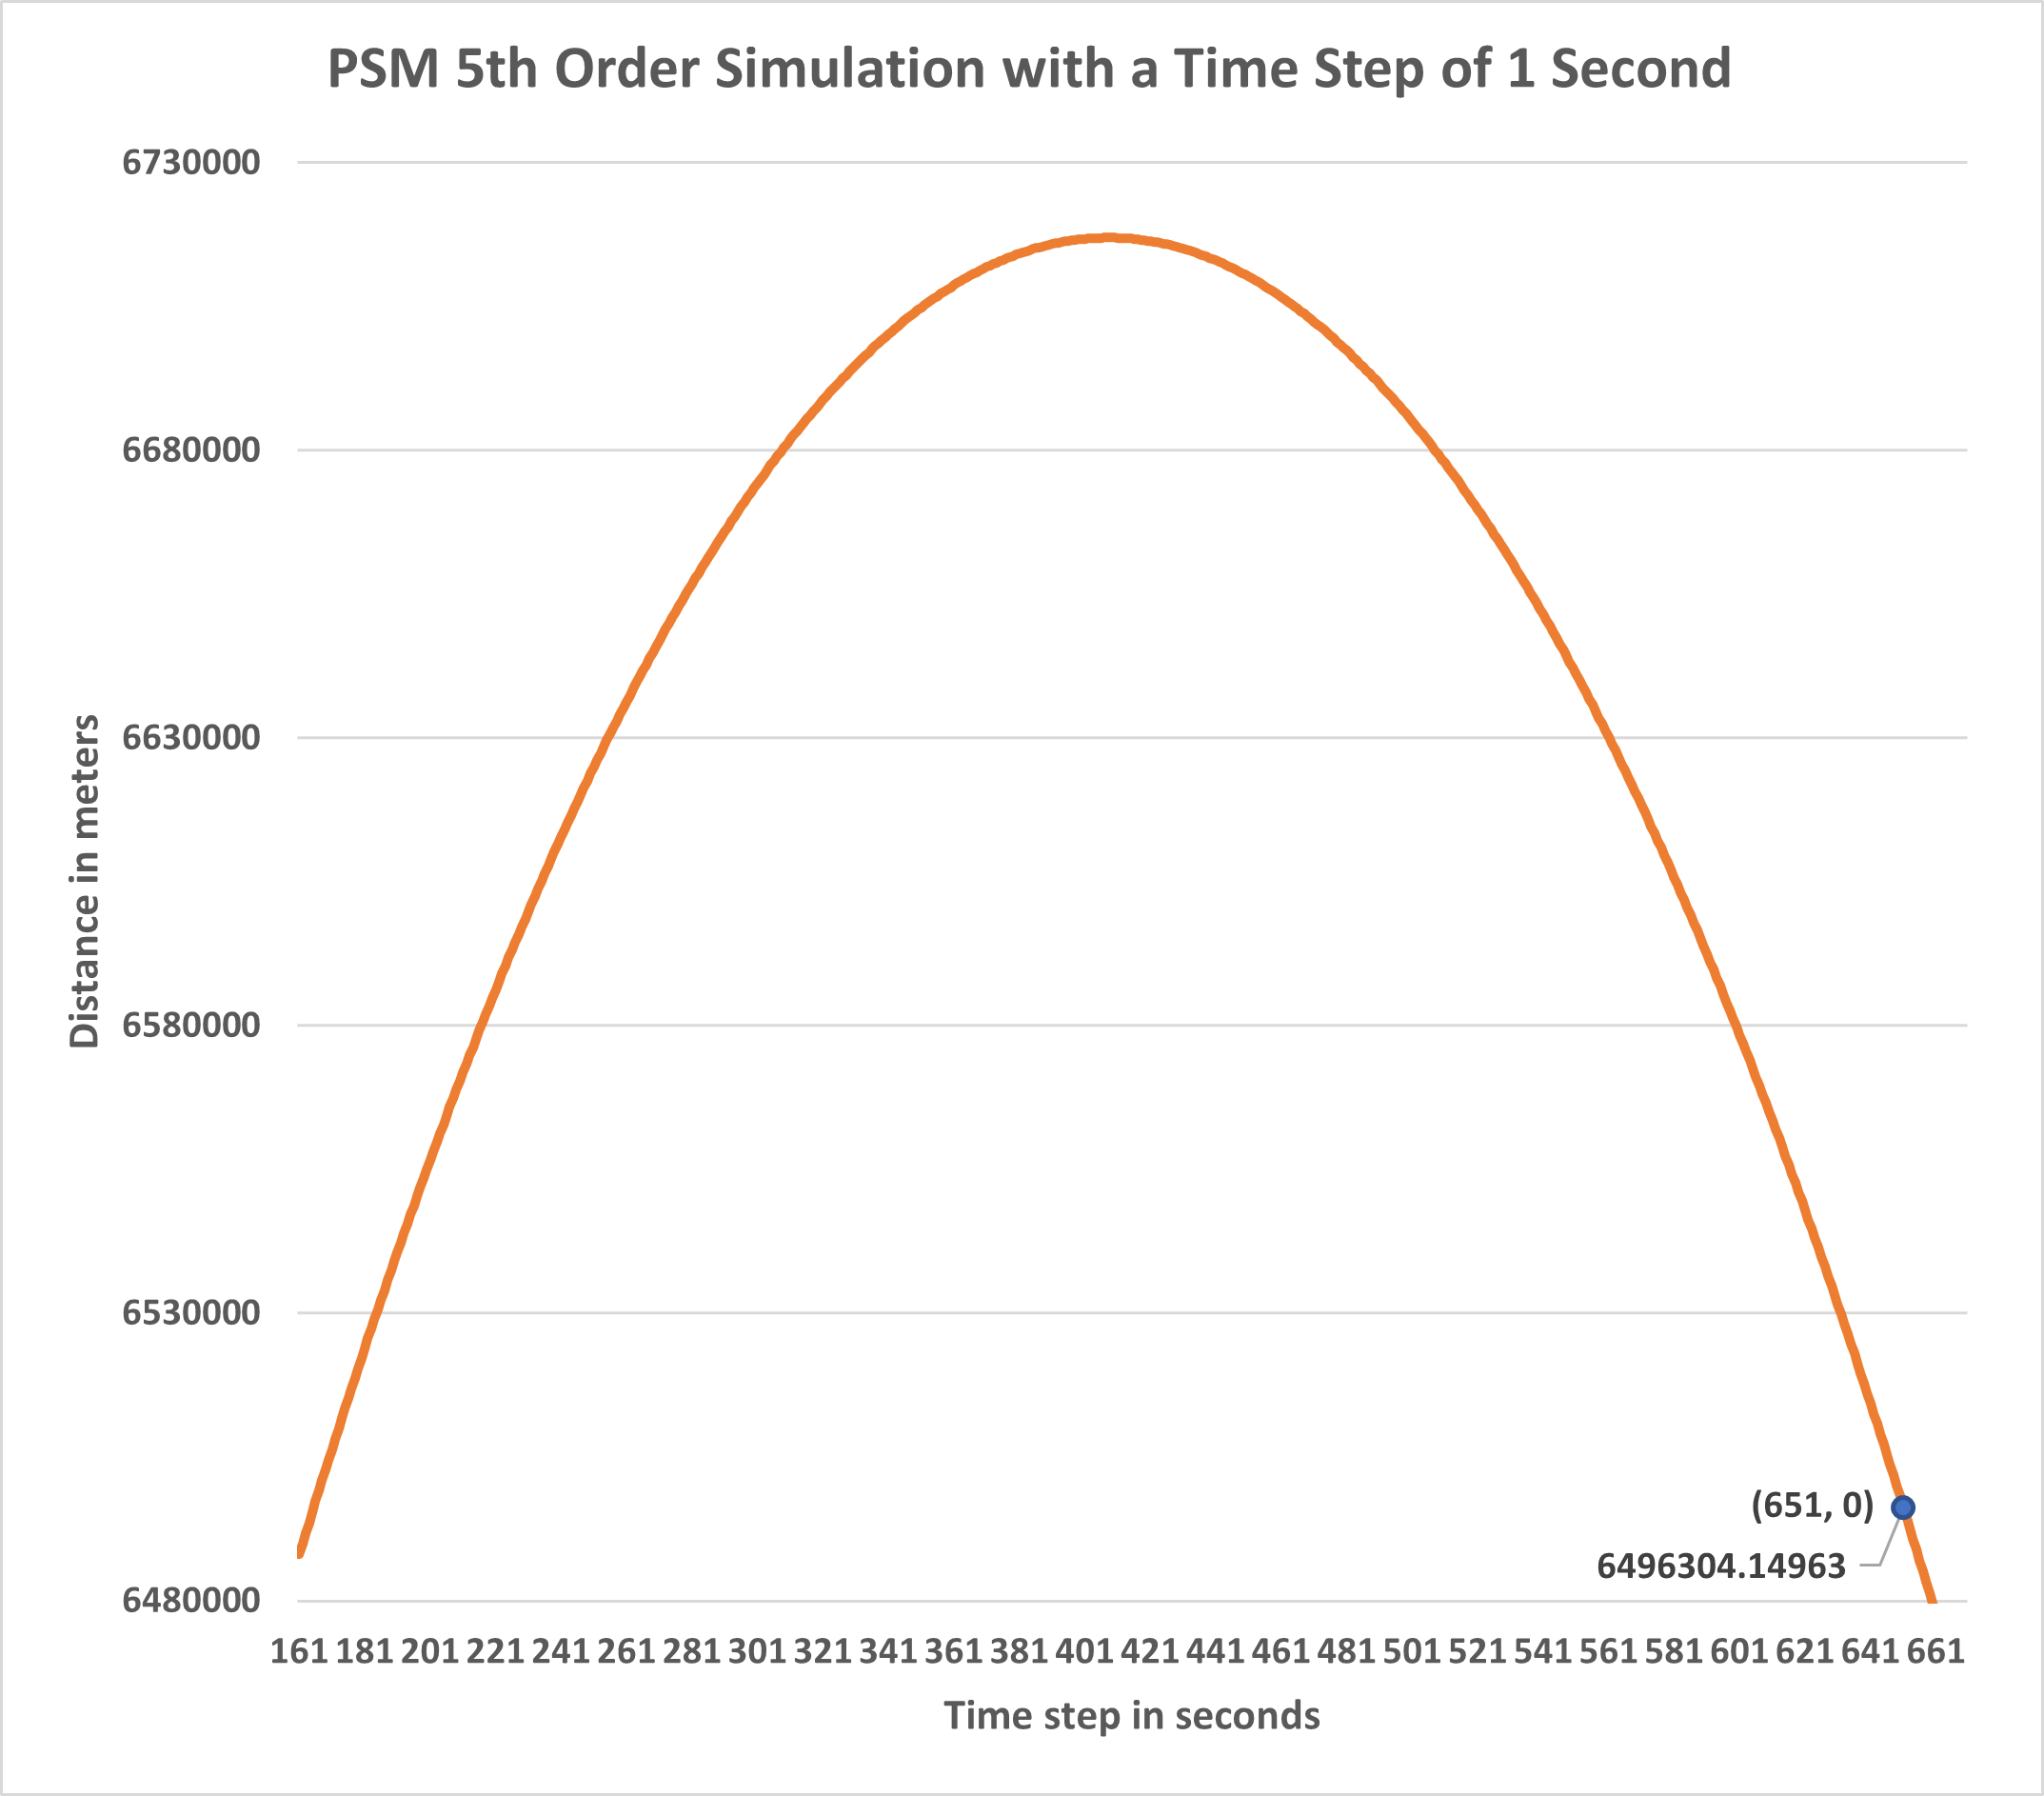
\includegraphics[width=0.16\textwidth]{images/PSM5 TS1 Plot.png}
        \end{tikzfigure}
    }
    \subcolumn{0.5}
    \block{Figure 2}
    {
        \begin{tikzfigure}
        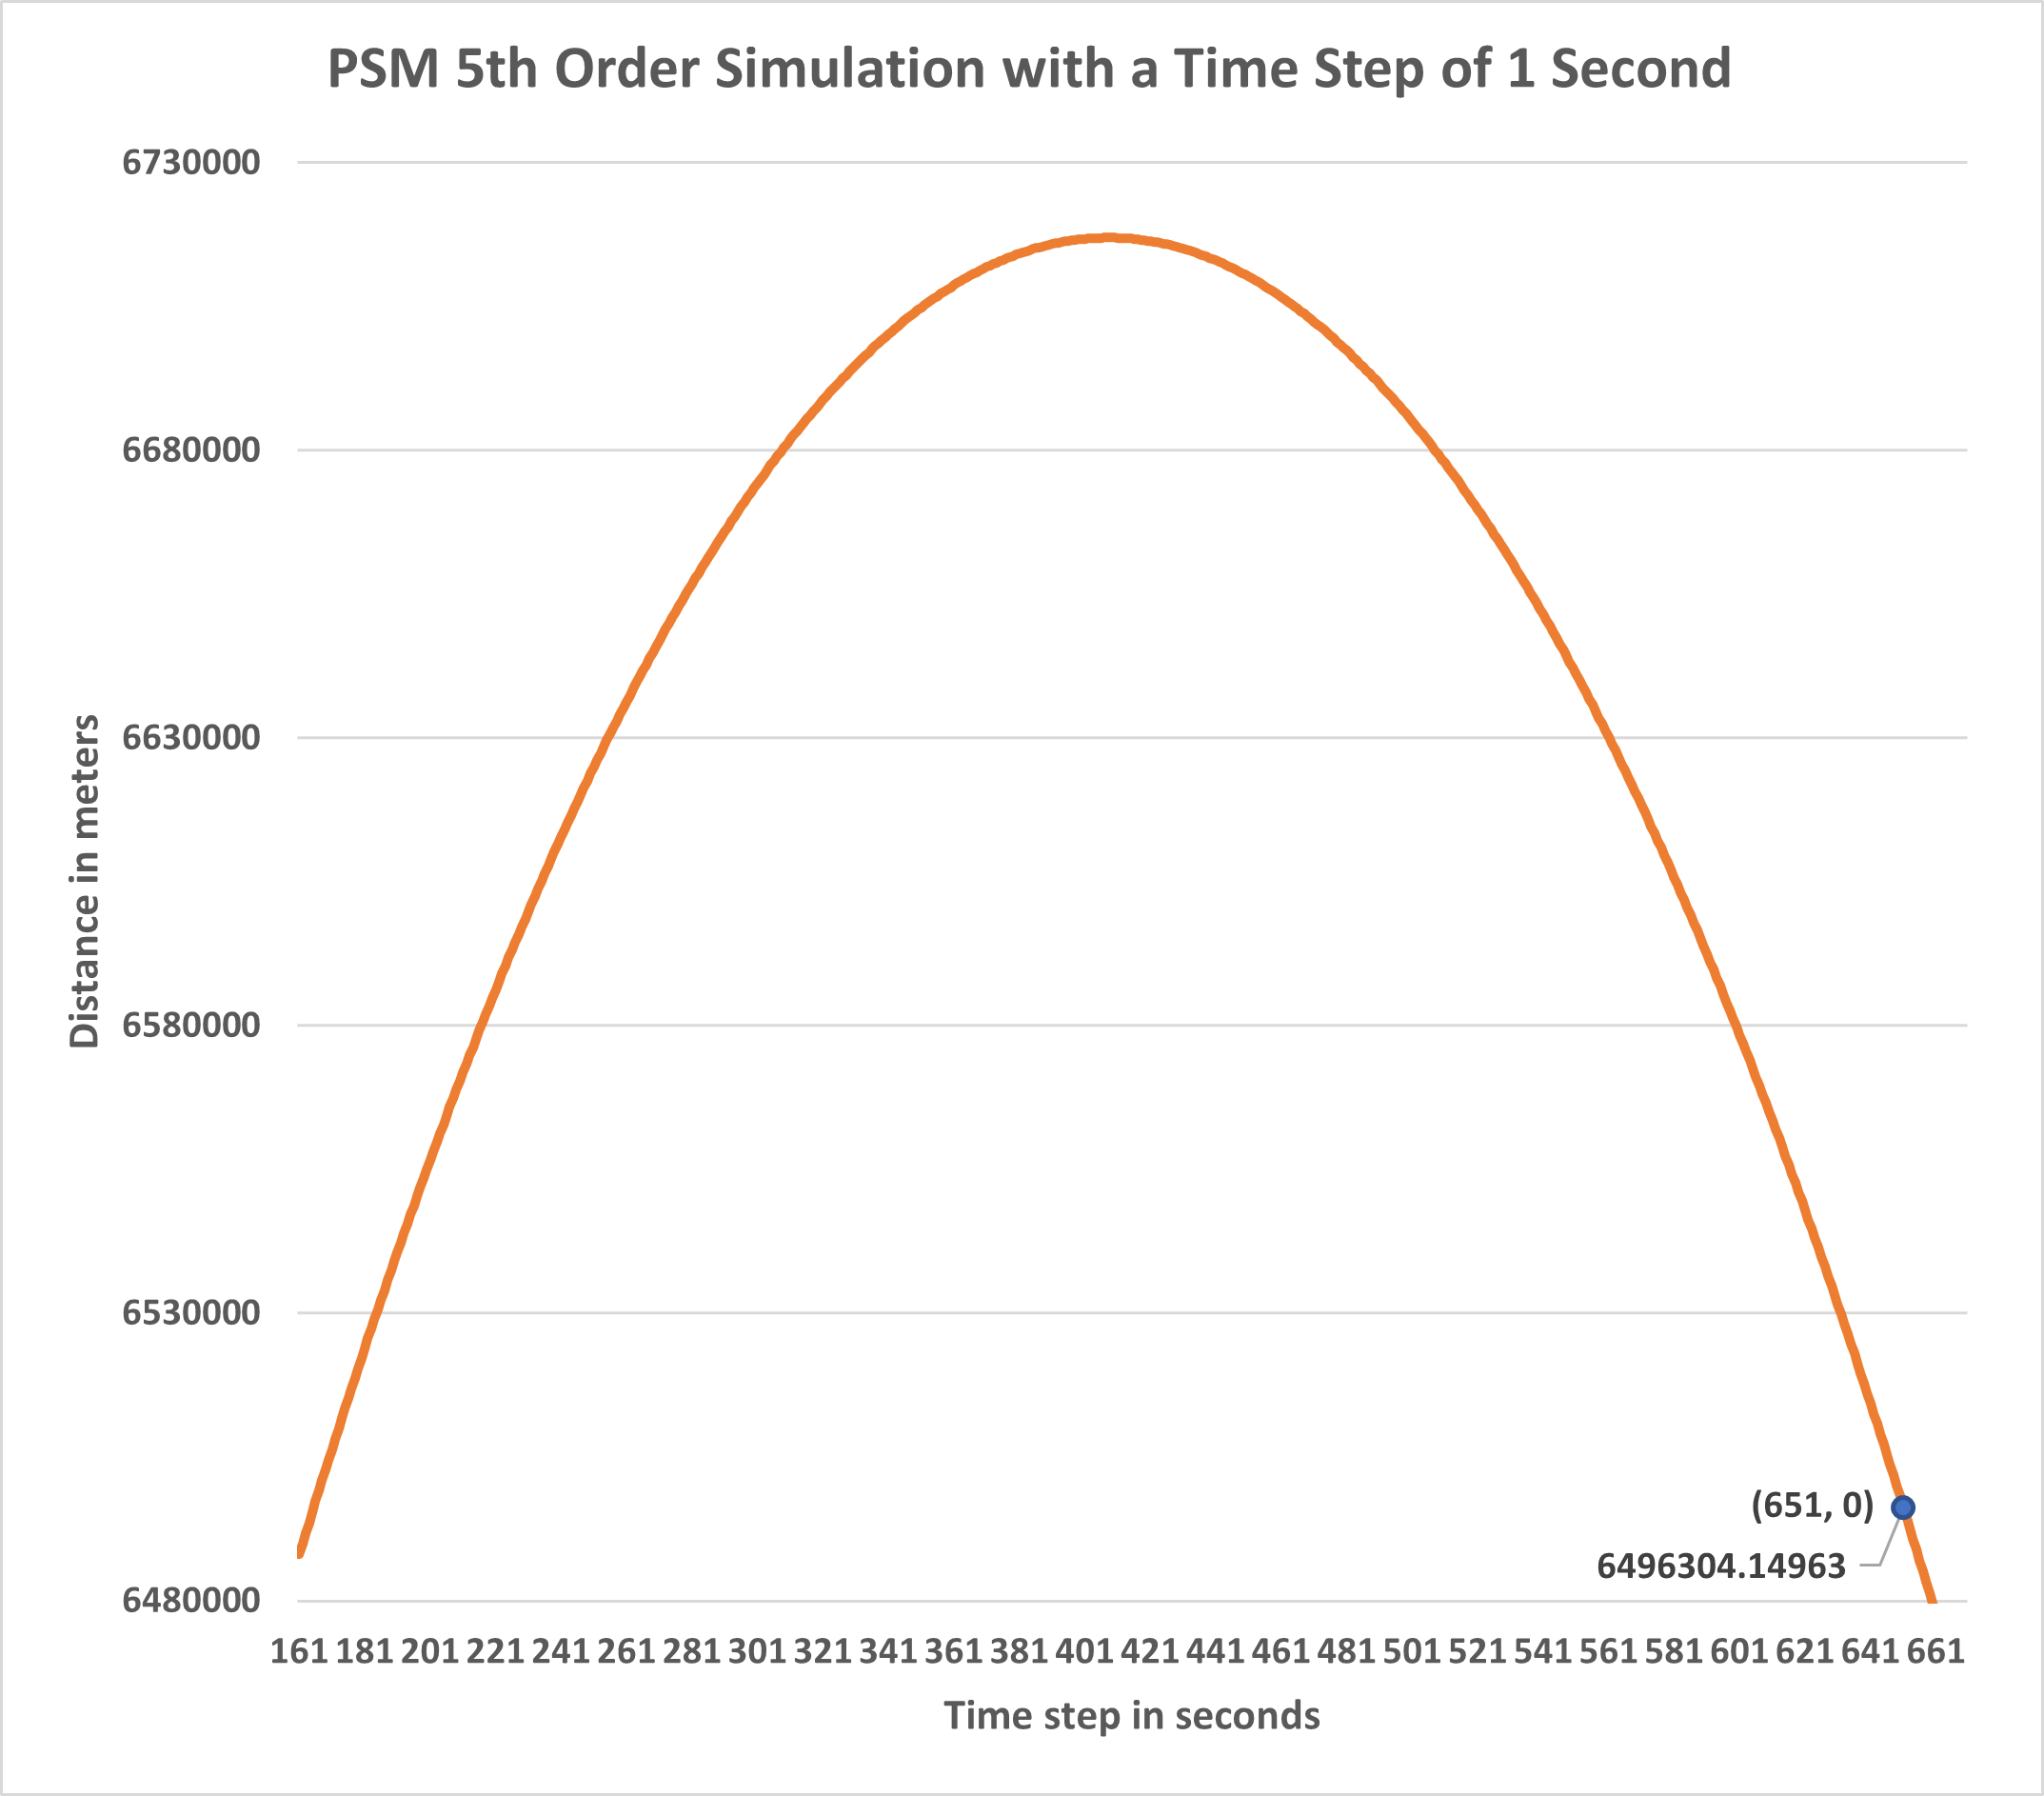
\includegraphics[width=0.16\textwidth]{images/PSM5 TS1 Plot.png}
        \end{tikzfigure}
    }
    \end{subcolumns}
    \block{Conclusion}
    {
        conclusion stuff
    }
    \column{0.45}
    \block{Cauchy Product Example Problem}
    {
        Use the power series method to solve $y^\prime = y^2$ ; $y(0) = -1$
        \begin{equation*}
            y = \sum\limits_{k=0}^{\infty}c_kt^k \Rightarrow y^\prime = \sum\limits_{k=1}^{\infty}kc_kt^{k-1}
        \end{equation*}
        Plug into $y^\prime = y^2$
        \begin{equation*}
            y^\prime = \sum\limits_{k=1}^{\infty}kc_kt^{k-1} = \left(\sum\limits_{k=0}^{\infty}c_kt^k\right) \left(\sum\limits_{k=0}^{\infty}c_kt^k\right)
        \end{equation*}
        Rewrite $y^2$ to match the form of the cauchy product
        \begin{equation}
            y^\prime = \sum\limits_{k=1}^{\infty}kc_kt^{k-1} = \sum\limits_{k=0}^{\infty} \underbrace{\left(\sum\limits_{j=0}^{k}c_jc_{k-j}\right)}_{\text{Cauchy product}}t^k
        \end{equation}
        Set $k = 1$ on both sides of the equation to solve for $c_k$
        \begin{equation*}
            y^\prime = \sum\limits_{k=1}^{\infty}kc_kt^{k-1} = \sum\limits_{k=1}^{\infty} \left(\sum\limits_{j=0}^{k-1}c_jc_{k-j-1}\right)t^{k-1}
        \end{equation*}
        \begin{equation}
            c_k = \frac{\sum\limits_{j=0}^{k-1}c_jc_{k-j-1}t^{k-1}}{k}
        \end{equation}
        Solving for $c_k$, we can see each coefficient is a function of previous coefficients
        \begin{equation*}
            \therefore c_1 = c_0c_0, c_2 = \frac{c_0c_1 + c_1c_0}{2}, c_3 = \frac{c_0c_2 + c_1c_1+ c_2c_0}{2},\dots
        \end{equation*}
    }
    \block{References}
    {
        Hello
    }
\end{columns}


\end{document}